% \documentclass[aspectratio=169,notes]{beamer}
\documentclass[aspectratio=169]{beamer}
\usetheme[faculty=phil]{fibeamer}
\usepackage{polyglossia}
\setmainlanguage{english} %% main locale instead of `english`, you
%% can typeset the presentation in either Czech or Slovak,
%% respectively.
\setotherlanguages{russian} %% The additional keys allow
%%
%%   \begin{otherlanguage}{czech}   ... \end{otherlanguage}
%%   \begin{otherlanguage}{slovak}  ... \end{otherlanguage}
%%
%% These macros specify information about the presentation
\title[Theoretical Mechanics]{Theoretical Mechanics, Lab 14: DYN VIRT DISP GEN EQN} %% that will be typeset on the
\subtitle{Principle of virtual displacements \\
General Equation of Dynamics (D'lambert-Lagrange) \\ \ } %% title page.
\author{Oleg Bulichev}
%% These additional packages are used within the document:
\usepackage{ragged2e}  % `\justifying` text
\usepackage{booktabs}  % Tables
\usepackage{tabularx}
\usepackage{tikz}      % Diagrams
\usetikzlibrary{calc, shapes, backgrounds}
\usepackage{amsmath, amssymb}
\usepackage{url}       % `\url`s
\usepackage{listings}  % Code listings
% \usepackage{subfigure}
\usepackage{floatrow}
\usepackage{subcaption}
\usepackage{mathtools}
\usepackage{todonotes}
\usepackage{fontspec}
\usepackage{multicol}
\usepackage{pdfpages}
\usepackage{wrapfig}
\usepackage{animate}
\usepackage{booktabs}
\usepackage{multirow}
% \usepackage{graphicx}
\usepackage{colortbl}
\usepackage{catchfilebetweentags}
\usepackage{makecell}
\graphicspath{{resources/}}
\frenchspacing

\setbeamertemplate{caption}[numbered]
\usetikzlibrary{graphs}

% \usepackage[backend=biber,style=ieee,autocite=footnote]{biblatex}
% \addbibresource{biblio.bib}
% \DefineBibliographyStrings{english}{%
%   bibliography = {References},}

\newcommand{\oleg}[2][] {\todo[color=red, #1] {OLEG:\\ #2}}
\newcommand{\fbckg}[1]{\usebackgroundtemplate{\includegraphics[width=\paperwidth]{#1}}}%frame background

\usepackage[framemethod=TikZ]{mdframed}
\newcommand{\dbox}[1]{
\begin{mdframed}[roundcorner=3pt, backgroundcolor=yellow, linewidth=0]
\vspace{1mm}
{#1}
\vspace{1mm}
\end{mdframed}
}

\begin{document}
\setlength{\abovedisplayskip}{0pt}
\setlength{\belowdisplayskip}{0pt}
\setlength{\abovedisplayshortskip}{0pt}
\setlength{\belowdisplayshortskip}{0pt}

\fbckg{fibeamer/figs/title_page.png}
\frame[c]{\setcounter{framenumber}{0}
    \usebeamerfont{title}%
    \usebeamercolor[fg]{title}%
    \begin{minipage}[b][6.5\baselineskip][b]{\textwidth}%
        \textcolor{black}{\raggedright\inserttitle}
    \end{minipage}
    % \vskip-1.5\baselineskip

    \usebeamerfont{subtitle}%
    \usebeamercolor[fg]{framesubtitle}%
    \begin{minipage}[b][3\baselineskip][b]{\textwidth}
        \raggedright%
        \insertsubtitle%
    \end{minipage}
    \vskip.25\baselineskip
}
%   \frame[c]{\maketitle}

\fbckg{fibeamer/figs/common.png}


\section*{Principle of virtual displacements}

\begin{frame}[t]{Principle of virtual displacements}
    \framesubtitle{}
    \scriptsize
        \begin{tabular}{>{\centering\arraybackslash} m{0.9cm}|>{\centering\arraybackslash} m{1cm}|>{\centering\arraybackslash} m{4.0cm}|>{\centering\arraybackslash} m{2.3cm}|>{\centering\arraybackslash} m{3.8cm} } 
            \toprule
            \toprule
           \textbf{ R. O.} & \textbf{Eqn \#} & \textbf{Equations} & \textbf{Applications} & \textbf{Extra Info} \\ 
            \hline
            \ExecuteMetaData[../../dynamics_methods_overview/dynamics_methods_overview]{sndpvd}
            \bottomrule
            \bottomrule
            \end{tabular}
    \end{frame}

\begin{frame}[t]{Task 1 (mine)}
\framesubtitle{}
    \begin{columns}[T,onlytextwidth]
        \begin{column}{0.59\textwidth}
            The platform structure consists of two frames connected by a rotation joint $C$. The left end of the frame $AC$ is rigidly fixed into the wall. the lower end of $CB$ is supported by cylindrical movable support $B$. 
            \medskip
            
            Determine the vertical support reaction $A$ under 
            the forces $P_1$ $P_2$.
        \end{column}
        \begin{column}{0.39\textwidth}
            \begin{figure}[H]
                \centering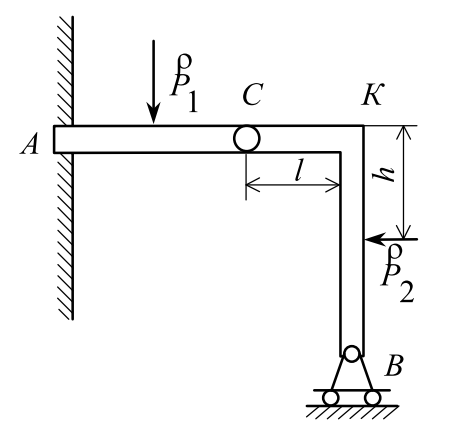
\includegraphics[height=6cm,width=1\textwidth,keepaspectratio]{image14.png}
                \label{fig:image14.png}
            \end{figure}
        \end{column}
    \end{columns}
\end{frame}

\begin{frame}[t]{Task 2 (yours): M (rus) 46.1}
\framesubtitle{}
    \begin{columns}[T,onlytextwidth]
        \begin{column}{0.59\textwidth}
            A weight $Q$ is lifted by means of a screw jack which is set in motion by a handle $OA=0.6$. A force $P=160$ is applied perpendicularly to the handle.
            \medskip

            Determine the magnitude of the weight $Q$, if the pitch of the screw thread is $h=0.012$.
            \bigskip

            \textit{Answer:} $Q=52200\ N$
        \end{column}
        \begin{column}{0.39\textwidth}
            \vspace{-0.6cm}
            \begin{figure}[H]
                \centering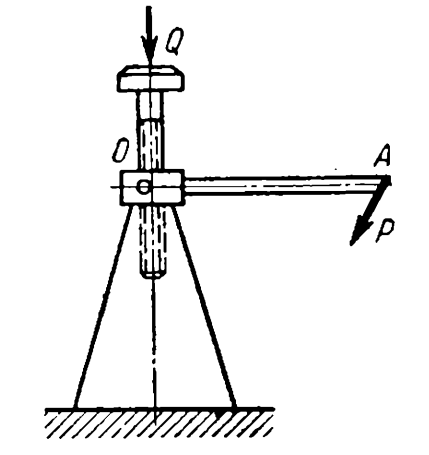
\includegraphics[height=6cm,width=1\textwidth,keepaspectratio]{image21.png}
                % \caption{caption_name}
                \label{fig:image21.png}
            \end{figure}
        \end{column}
    \end{columns}
\end{frame}

\section*{General Equation of Dynamics}

\begin{frame}[t]{General Equation of Dynamics}
    \framesubtitle{}
    \scriptsize
        \begin{tabular}{>{\centering\arraybackslash} m{0.9cm}|>{\centering\arraybackslash} m{2cm}|>{\centering\arraybackslash} m{4.0cm}|>{\centering\arraybackslash} m{2.3cm}|>{\centering\arraybackslash} m{2.8cm} } 
            \toprule
            \toprule
           \textbf{ R. O.} & \textbf{Eqn \#} & \textbf{Equations} & \textbf{Applications} & \textbf{Extra Info} \\ 
            \hline
            \ExecuteMetaData[../../dynamics_methods_overview/dynamics_methods_overview]{sndgeneqndyn}
            \bottomrule
            \bottomrule
            \end{tabular}
    \end{frame}

\begin{frame}[t]{Task 3 (mine)}
\framesubtitle{}
\small
\begin{columns}[T,onlytextwidth]
    \begin{column}{0.59\textwidth}
        A load $A$ of weight $P$ moves down on a weightless inextensible thread which first runs over a fixed weightless pulley $D$ and the coils on a sheave $B$, thus forcing the shaft $C$ to roll without sliding along a horizontal rail.
        \medskip

        The sheave $B$ of radius $R$ is mounted tightly on the shaft $C$ of radius $R$: the total weight of the sheave $B$ and the shaft $C$ is $Q$.
        \medskip

        The axis $O$ is perpendicular to the plane of the drawing and the radius of gyration relative to $O$ is $\rho$.

        \bigskip
        Find the acceleration of the load $A$.

    \end{column}
    \begin{column}{0.39\textwidth}
            \begin{figure}[H]
        \centering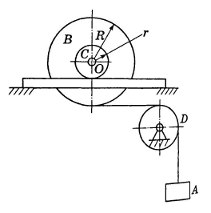
\includegraphics[height=6cm,width=1\textwidth,keepaspectratio]{image11.png}
        \label{fig:image11.png}
    \end{figure}
    \end{column}
\end{columns}
\end{frame}

\begin{frame}[t]{Task 4 (yours): M (rus) 47.5}
    \framesubtitle{}
        \begin{columns}[T,onlytextwidth]
            \begin{column}{0.59\textwidth}
                To the system of blocks shown in the figure are suspended weights $M_1=10\ kg$ and $M_2=8$.
                \medskip
                
                Determine the acceleration $a_2$ of the weight $M_2$ and the tension of the thread, neglecting the masses of the blocks.
                \bigskip

                \textit{Answer:} $a_2 = 2.9\ \frac{m}{s^2},\ T=56\ N$
            \end{column}
            \begin{column}{0.39\textwidth}
                \begin{figure}[H]
                    \centering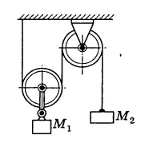
\includegraphics[height=4cm,width=1\textwidth,keepaspectratio]{image22.png}
                    % \caption{caption_name}
                    \label{fig:image22.png}
                \end{figure}
            \end{column}
        \end{columns}
    \end{frame}

\fbckg{fibeamer/figs/last_page.png}
\frame[plain]{}
\end{document}